%%%%%%%%%%%%%%%%%%%%%%%%%%%%%%%%%%%%%%%%%
% Beamer Presentation
% LaTeX Template
% Version 1.0 (10/11/12)
%
% This template has been downloaded from:
% http://www.LaTeXTemplates.com
%
% License:
% CC BY-NC-SA 3.0 (http://creativecommons.org/licenses/by-nc-sa/3.0/)
%
%%%%%%%%%%%%%%%%%%%%%%%%%%%%%%%%%%%%%%%%%

%----------------------------------------------------------------------------------------
%	PACKAGES AND THEMES
%----------------------------------------------------------------------------------------

\documentclass[10pt]{beamer}

\mode<presentation> {

% The Beamer class comes with a number of default slide themes
% which change the colors and layouts of slides. Below this is a list
% of all the themes, uncomment each in turn to see what they look like.

%\usetheme{default}
%\usetheme{AnnArbor}
%\usetheme{Antibes}
%\usetheme{Bergen}
%\usetheme{Berkeley}
%\usetheme{Berlin}
%\usetheme{Boadilla}
%\usetheme{CambridgeUS}
%\usetheme{Copenhagen}
%\usetheme{Darmstadt}
%\usetheme{Dresden}
%\usetheme{Frankfurt}
%\usetheme{Goettingen}
%\usetheme{Hannover}
%\usetheme{Ilmenau}
%\usetheme{JuanLesPins}
%\usetheme{Luebeck}
\usetheme{Madrid}
%\usetheme{Malmoe}
%\usetheme{Marburg}
%\usetheme{Montpellier}
%\usetheme{PaloAlto}
%\usetheme{Pittsburgh}
%\usetheme{Rochester}
%\usetheme{Singapore}
%\usetheme{Szeged}
%\usetheme{Warsaw}

% As well as themes, the Beamer class has a number of color themes
% for any slide theme. Uncomment each of these in turn to see how it
% changes the colors of your current slide theme.

%\usecolortheme{albatross}
%\usecolortheme{beaver}
%\usecolortheme{beetle}
%\usecolortheme{crane}
%\usecolortheme{dolphin}
%\usecolortheme{dove}
%\usecolortheme{fly}
%\usecolortheme{lily}
%\usecolortheme{orchid}
%\usecolortheme{rose}
%\usecolortheme{seagull}
%\usecolortheme{seahorse}
%\usecolortheme{whale}
%\usecolortheme{wolverine}

%\setbeamertemplate{footline} % To remove the footer line in all slides uncomment this line
%\setbeamertemplate{footline}[page number] % To replace the footer line in all slides with a simple slide count uncomment this line

%\setbeamertemplate{navigation symbols}{} % To remove the navigation symbols from the bottom of all slides uncomment this line
}

\usepackage{graphicx} % Allows including images
\usepackage{booktabs} % Allows the use of \toprule, \midrule and \bottomrule in tables
\usepackage{hyperref}
\usepackage{tikz}
\usepackage{algpseudocode}
\usepackage{algorithm}
\usepackage{multicol}
\usepackage[utf8]{inputenc}
\setbeamerfont{frametitle}{size=\large}
\setbeamerfont{framesubtitle}{size=\small}
\setbeamertemplate{caption}[numbered]
\usepackage{amsmath}
\DeclareMathOperator*{\argmax}{arg\,max}
\DeclareMathOperator*{\argmin}{arg\,min}

%----------------------------------------------------------------------------------------
%	TITLE PAGE
%----------------------------------------------------------------------------------------

\title[Advanced Machine Learning]{Advanced Machine Learning} % The short title appears at the bottom of every slide, the full title is only on the title page
\subtitle{\textbf{Paper:} Shwartz-Ziv et al., \textit{Opening the Black Box of Deep Neural Networks via Information} \cite{Tishby3, Tishby1, Tishby2}}
\author[Gandara V. Eduardo and Werenne Aurélien]{Gandara V. Eduardo and Werenne Aurélien} 
\institute[ULiège] 
{
University of Li\`{e}ge \\ 
}
\date{\today} 

\begin{document}

\begin{frame}
\titlepage 
\end{frame}

\begin{frame}
\frametitle{Overview} 
\tableofcontents 
\end{frame}

%----------------------------------------------------------------------------------------
%	PRESENTATION SLIDES
%----------------------------------------------------------------------------------------

%------------------------------------------------
\section{Background} 
%------------------------------------------------

\begin{frame}
\frametitle{Overview}
\tableofcontents[currentsection,subsectionstyle=shaded]
\end{frame}

%------------------------------------------------
\begin{frame}
\frametitle{Background}
\framesubtitle{Information theory}
\begin{multicols}{2}
\begin{itemize}
\uncover<1-3>{\item \textbf{Information} $$I(X) = - \log{p(x)}$$\\[0.25cm]}
\uncover<2-3>{\item \textbf{Entropy} $$H(X) = - \sum_{x \in \mathbb{X}} p(x)\log{p(x)}$$\\[0.25cm]}
\uncover<3-3>{\item \textbf{Mutual Information} $$I(X;Y) = H(X) - H(X | Y)$$}
\end{itemize}
\columnbreak
\uncover<3-3>{\begin{figure}
\vspace*{1.2mm}
\centering

\includegraphics[scale=0.28]{figs/venn-diagram.png}
\end{figure}}
\end{multicols}
\end{frame}

%------------------------------------------------
\begin{frame}
\frametitle{Background}
\framesubtitle{Digital Processing Inequality}
\begin{itemize}
\item \textbf{Digital Processing Inequality:} \\[0.5cm]
For a Markov Chain of the following form,
\begin{figure}
\vspace*{2mm}
\centering
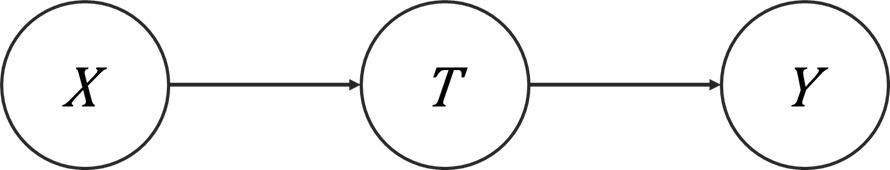
\includegraphics[scale=0.18]{figs/dpi.jpeg}
\end{figure}
\vspace*{2mm}
the inequality $I(X;T) \geq I(X;Y)$ is valid.
\end{itemize}
\end{frame}

%------------------------------------------------
\begin{frame}
\frametitle{Background}
\framesubtitle{Information Bottleneck}
\begin{itemize}
\item \textbf{Minimal Sufficient Statistics:} $$ T(x) = \argmin_{S(X):\, I(S(X);Y) \,=\, I(X;Y)} I(S(X);X)$$\\[0.25cm]
which can be rewritten with as the following Lagrangian, $$ \min_{p(x),p(y|t),p(t)} I(X;T) - \beta I(T;Y)$$
\end{itemize}
\end{frame}

%------------------------------------------------
\section{Opening the black box} 
%------------------------------------------------

\begin{frame}
\frametitle{Overview}
\tableofcontents[currentsection,subsectionstyle=shaded]
\end{frame}

%------------------------------------------------
\begin{frame}
\frametitle{Opening the black box}
\framesubtitle{Main idea}
\begin{figure}
\centering
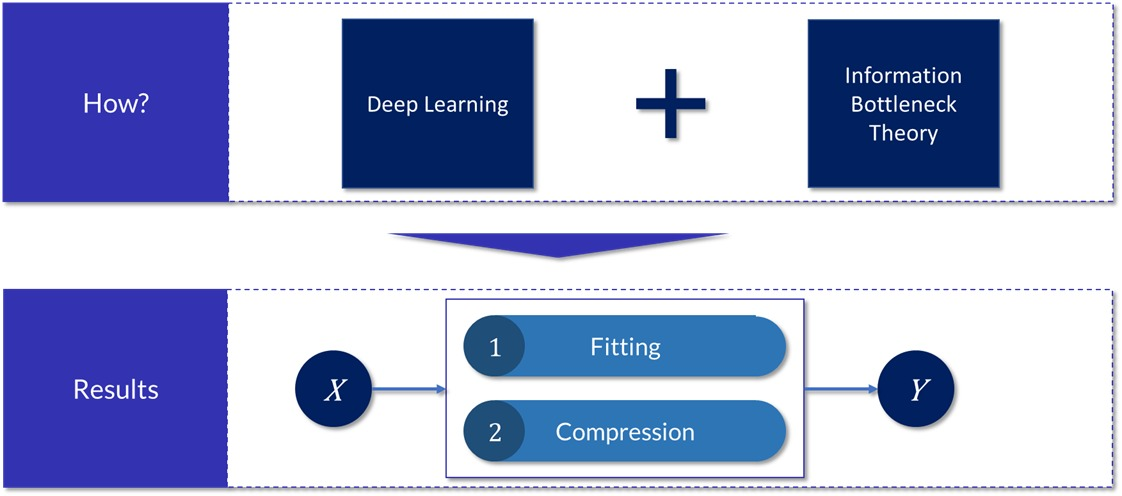
\includegraphics[scale=0.30]{figs/main-idea.jpeg}
\end{figure}
\end{frame}

%------------------------------------------------
\begin{frame}
\frametitle{Opening the black box}
\framesubtitle{Framework}
\begin{figure}
\centering
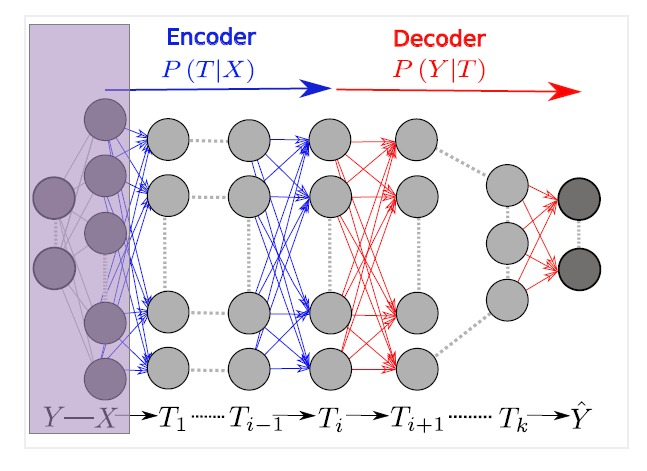
\includegraphics[scale=0.37]{figs/markov-chain-nn.jpeg}
\end{figure}
\vspace*{-4.5mm}
\begin{center}
Supervised Deep Learning $\stackrel{?}{=} \min \{I(X;T) - \beta I(T;Y)\} $
\end{center}
\end{frame}

%------------------------------------------------
\begin{frame}
\frametitle{Opening the black box}
\framesubtitle{Information Plane}
\begin{itemize}
\item Information plane (\href{https://youtu.be/XL07WEc2TRI?t=1333}{\textcolor{blue}{video}})
\end{itemize}
\begin{figure}
\centering
\vspace*{-1.8mm}
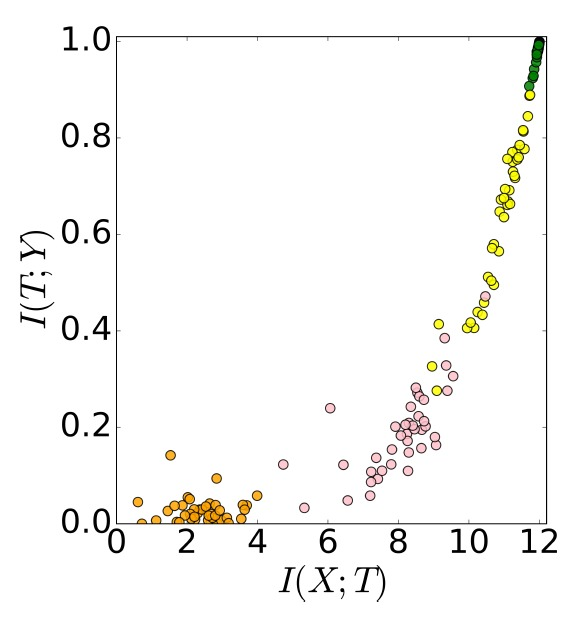
\includegraphics[scale=0.28]{figs/initial-information-plane.jpeg}
\end{figure}
\end{frame}

%------------------------------------------------
\begin{frame}
\frametitle{Opening the black box}
\framesubtitle{Norm and Variance of Gradients}
\begin{figure}
\centering
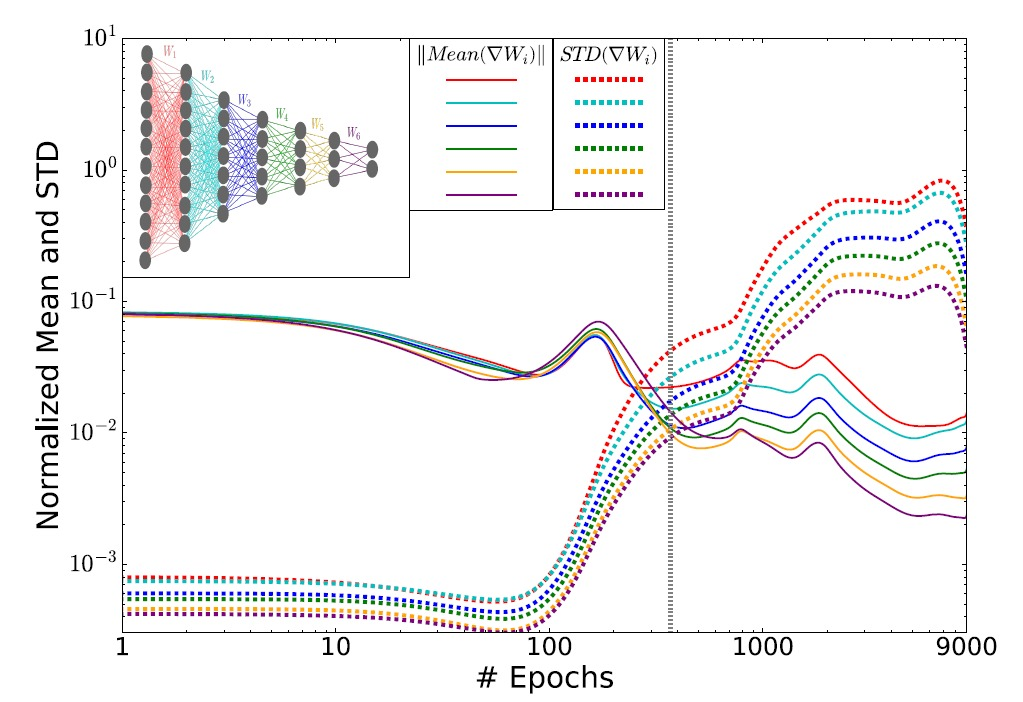
\includegraphics[scale=0.3]{figs/gradients.jpeg}
\end{figure}
\end{frame}

%------------------------------------------------
\begin{frame}
\frametitle{Opening the black box}
\framesubtitle{Flat Minima}
Continuing SGD in local minima can be modelled as a Random Walk!
\begin{figure}
\vspace*{4mm}
\centering
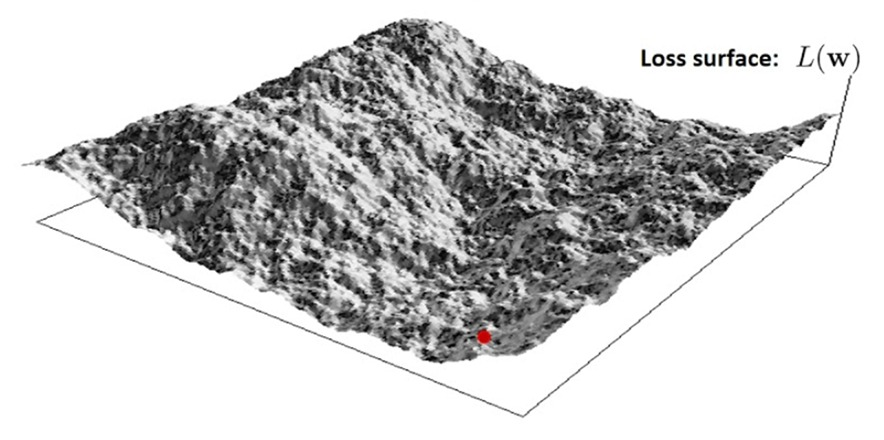
\includegraphics[scale=0.35]{figs/flat-loss.jpeg}
\end{figure}
\end{frame}

%------------------------------------------------
\begin{frame}
\frametitle{Opening the black box}
\framesubtitle{Diffusion}
Why can a \href{https://www.wolframalpha.com/input/?i=randomwalk}{\textcolor{blue}{Random Walk}} be seen as a compression?\\[0.35cm]
\uncover<2-4>{$\Rightarrow$ Increases entropy of weights}\\[0.2cm]
\uncover<3-4>{$\Rightarrow$ Maximizes $H(X|T_i)$}\\[0.2cm]
\uncover<4-4>{$\Rightarrow$ Minimizes $I(X;T_i) = \underbrace{H(X)}_{constant} - H(X|T_i)$}
\end{frame}

%------------------------------------------------
\begin{frame}
\frametitle{Opening the black box}
\framesubtitle{Underfitting \& overfitting}
\begin{itemize}
\item Evolution in the information plane, for different training sample sizes. From left to right (5\% of the data, 45\% of the data, 85\% of the data).
\end{itemize}
\begin{figure}
\centering
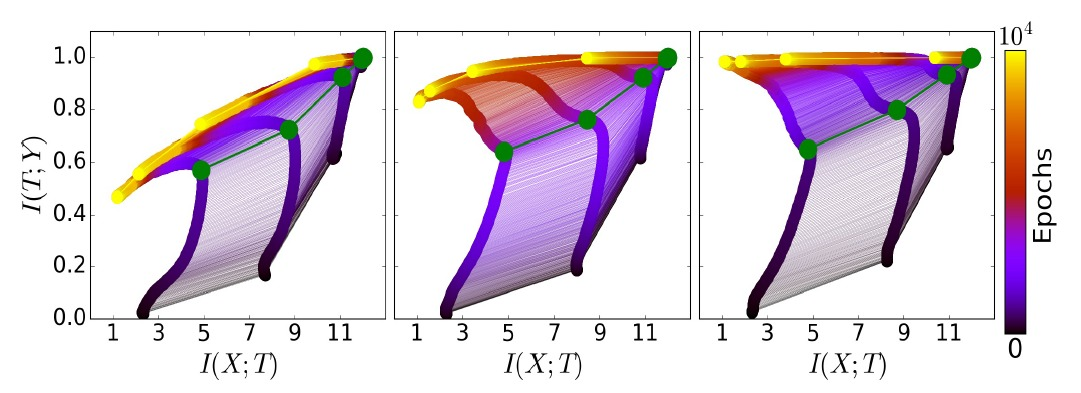
\includegraphics[scale=0.3]{figs/overfitting.jpeg}
\end{figure}
\end{frame}

%------------------------------------------------
\begin{frame}
\frametitle{Opening the black box}
\framesubtitle{Hidden Layers}
\vspace*{-1.5mm}
\begin{figure}
\centering
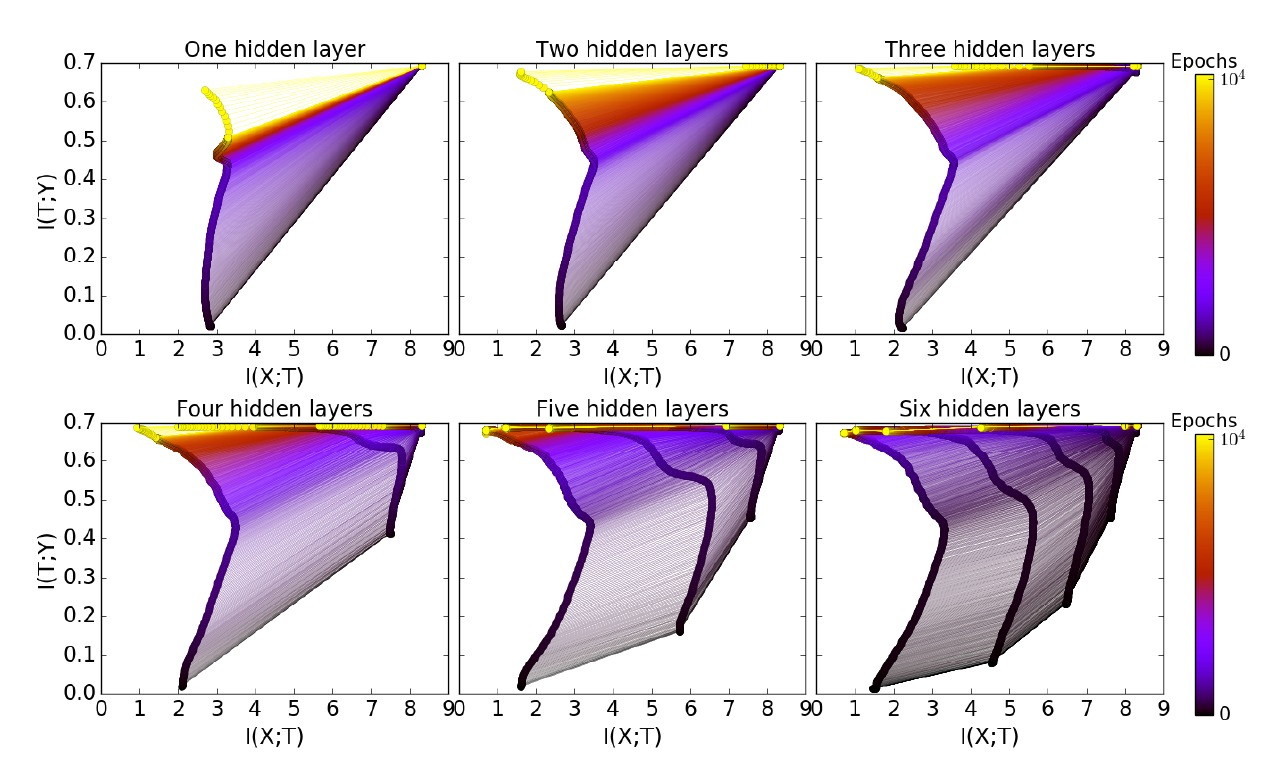
\includegraphics[scale=0.23]{figs/hidden-layers.jpeg}
\end{figure}
\begin{center}
Why? $ \Rightarrow \boxed{exp(\sum_k \Delta I_X^k) \gg \sum_k exp(\Delta I_X^k)} $
\end{center}
\end{frame}

%------------------------------------------------
\begin{frame}
\frametitle{Opening the black box}
\framesubtitle{IB Curve}
\begin{center}
Supervised Deep Learning $\approx \min \{I(X;T) - \beta I(T;Y)\} $
\end{center}
\begin{figure}
\centering
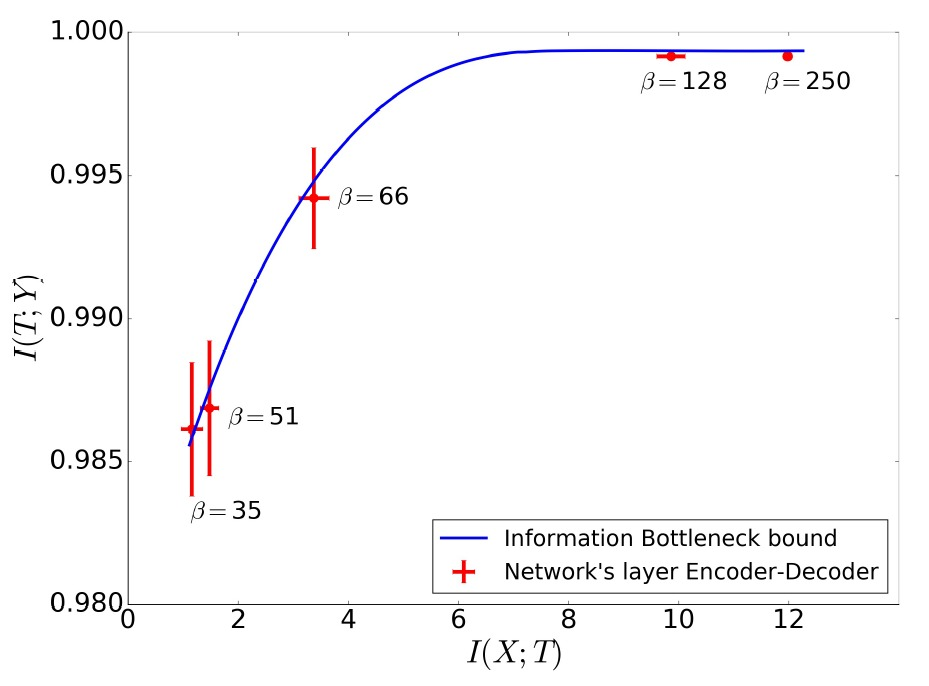
\includegraphics[scale=0.23]{figs/ib-curve.jpeg}
\end{figure}
\end{frame}

%------------------------------------------------
\begin{frame}
\frametitle{Opening the black box}
\framesubtitle{Summary}
\begin{itemize}
\item Fitting then Compressing
\item Overfitting = Overcompression
\item Noise of SGD $\Rightarrow$ Generalization
\item Do we need to adapt \textit{Early Stopping} method? 
\end{itemize}
\vspace*{-1.5mm}
\begin{figure}
\centering
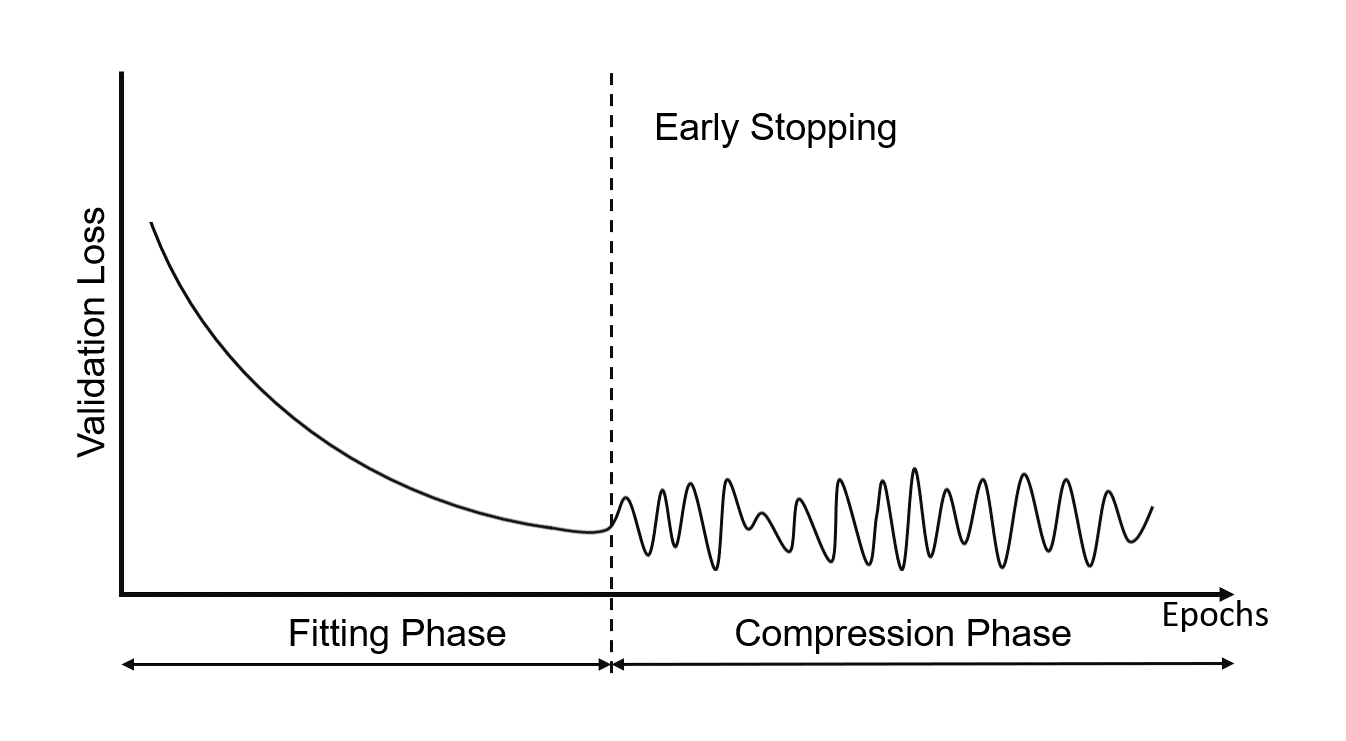
\includegraphics[scale=0.32]{figs/early-stopping.png}
\end{figure}
\end{frame}

%------------------------------------------------
\section{Discussion} 
%------------------------------------------------

\begin{frame}
\frametitle{Overview}
\tableofcontents[currentsection,subsectionstyle=shaded]
\end{frame}

%------------------------------------------------
\begin{frame}
\frametitle{Discussion}
\framesubtitle{Controversy}
\begin{figure}
\centering
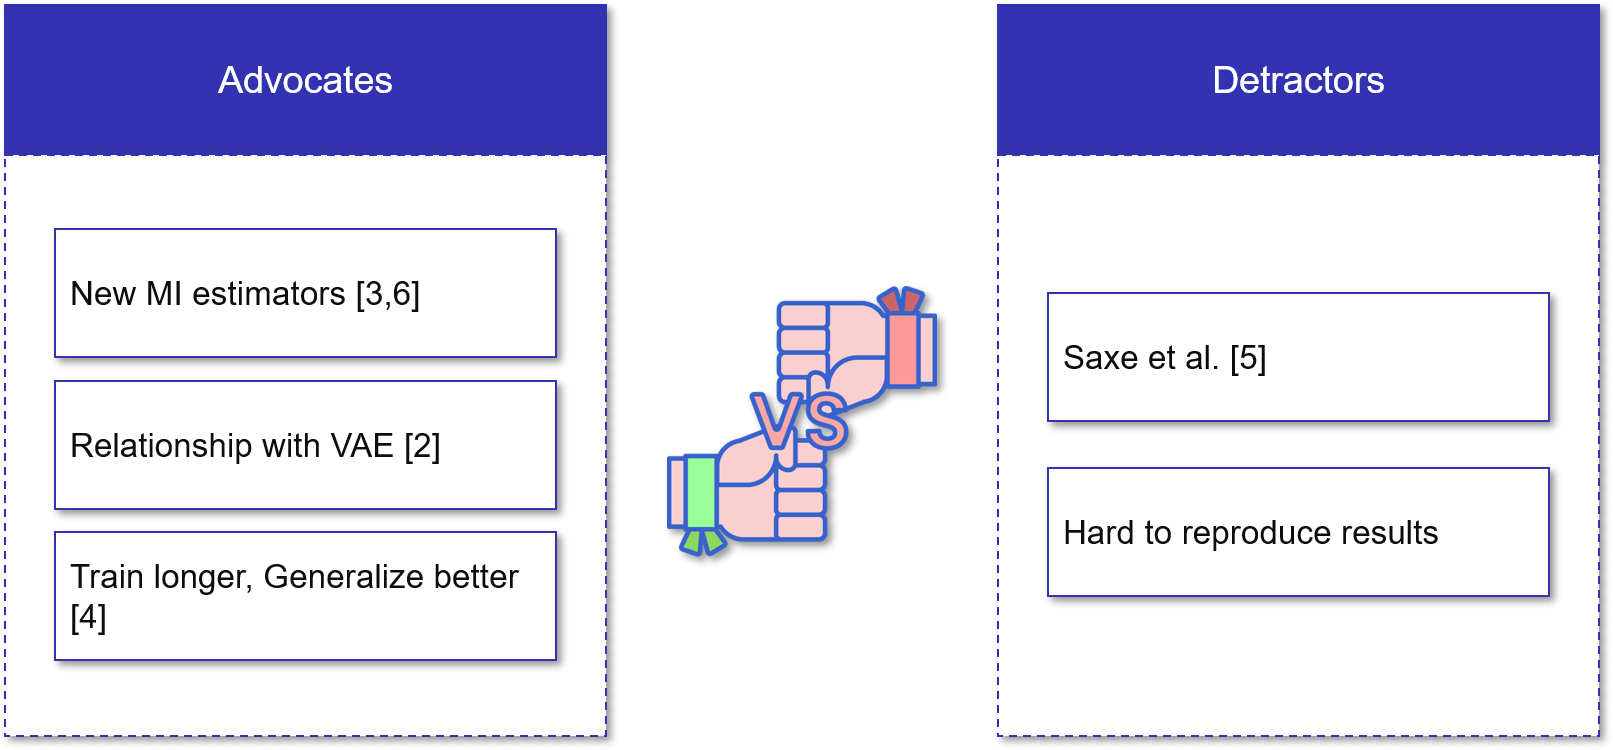
\includegraphics[scale=0.4]{figs/vs2.png}
\end{figure}
\end{frame}

%------------------------------------------------
\begin{frame}
\frametitle{Discussion}
\framesubtitle{Pros and cons}
%Pros and cons:\\[0.2cm]
Pros:\\
    \begin{itemize}
        \item[\checkmark] New insight of how DL works
        \item[\checkmark] Led to various applications \cite{information-dropout, vib}
        \item[\checkmark] Justified Mathematically
        \item[\checkmark] Available code
        \\[0.5cm]
    \end{itemize}
Cons:\\
     \begin{itemize}
        \item[$\times$] Estimating MI is computationally expensive
        \item[$\times$] Not tested on non-saturating functions and large networks
        \item[$\times$] No verification of the results on challenging datasets
    \end{itemize}
\end{frame}


%----------------------------------------------------------------------------------------
\section*{References}
\phantom{\cite{MI1, MI2, saxe, train-longer}}
\frametitle{References}
\bibliographystyle{plain}
\bibliography{bibliography}

\end{document}
